\documentclass[11pt,letterpaper]{article}
\usepackage[utf8]{inputenc}
\usepackage[T1]{fontenc}
\usepackage[spanish]{babel}
\usepackage{amsmath}
\usepackage{amsfonts}
\usepackage{amssymb}
\usepackage{graphicx}
\usepackage{lmodern}
\usepackage{xspace}
\usepackage{multicol}
\usepackage{hyperref}
\usepackage{float}
\usepackage{hyperref}
\usepackage{color}
\usepackage{framed}
\usepackage{pdfpages}



\usepackage[left=2cm,right=2cm,top=2cm,bottom=2cm]{geometry}

\newcommand{\X}{\mathbb{X}}
\newcommand{\x}{\mathbf{x}}
\newcommand{\Y}{\mathbf{Y}}
\newcommand{\y}{\mathbf{y}}
\newcommand{\xbarn}{\bar{x}_n}
\newcommand{\ybarn}{\bar{y}_n}
\newcommand{\paren}[1]{\left( #1 \right)}
\newcommand{\llaves}[1]{\left\lbrace #1 \right\rbrace}
\newcommand{\barra}{\,\vert\,}
\newcommand{\mP}{\mathbb{P}}
\newcommand{\mE}{\mathbb{E}}
\newcommand{\mR}{\mathbb{R}}
\newcommand{\mJ}{\mathbf{J}}
\newcommand{\mX}{\mathbf{X}}
\newcommand{\mS}{\mathbf{S}}
\newcommand{\mA}{\mathbf{A}}
\newcommand{\unos}{\boldsymbol{1}}
\newcommand{\xbarnv}{\bar{\mathbf{x}}_n}
\newcommand{\abs}[1]{\left\vert #1 \right\vert}
\newcommand{\muv}{\boldsymbol{\mu}}
\newcommand{\mcov}{\boldsymbol{\Sigma}}
\newcommand{\vbet}{\boldsymbol{\beta}}
\newcommand{\veps}{\boldsymbol{\epsilon}}
\newcommand{\mcC}{\mathcal{C}}
\newcommand{\mcR}{\mathcal{R}}
\newcommand{\mcN}{\mathcal{N}}

\newcommand{\ceros}{\boldsymbol{0}}
\newcommand{\mH}{\mathbf{H}}
\newcommand{\ve}{\mathbf{e}}
\newcommand{\avec}{\mathbf{a}}
\newcommand{\res}{\textbf{RESPUESTA}\\}

\newcommand{\defi}[3]{\textbf{Definición:#3}}
\newcommand{\fin}{$\blacksquare.$}
\newcommand{\finf}{\blacksquare.}
\newcommand{\tr}{\text{tr}}
\newcommand*{\temp}{\multicolumn{1}{r|}{}}

\newcommand{\grstep}[2][\relax]{%
   \ensuremath{\mathrel{
       {\mathop{\longrightarrow}\limits^{#2\mathstrut}_{
                                     \begin{subarray}{l} #1 \end{subarray}}}}}}
\newcommand{\swap}{\leftrightarrow}

\newcommand{\gen}{\text{gen}}
\newtheorem{thmt}{Teorema:}
\newtheorem{thmd}{Definición:}
\newtheorem{thml}{Lema:}

\begin{document}
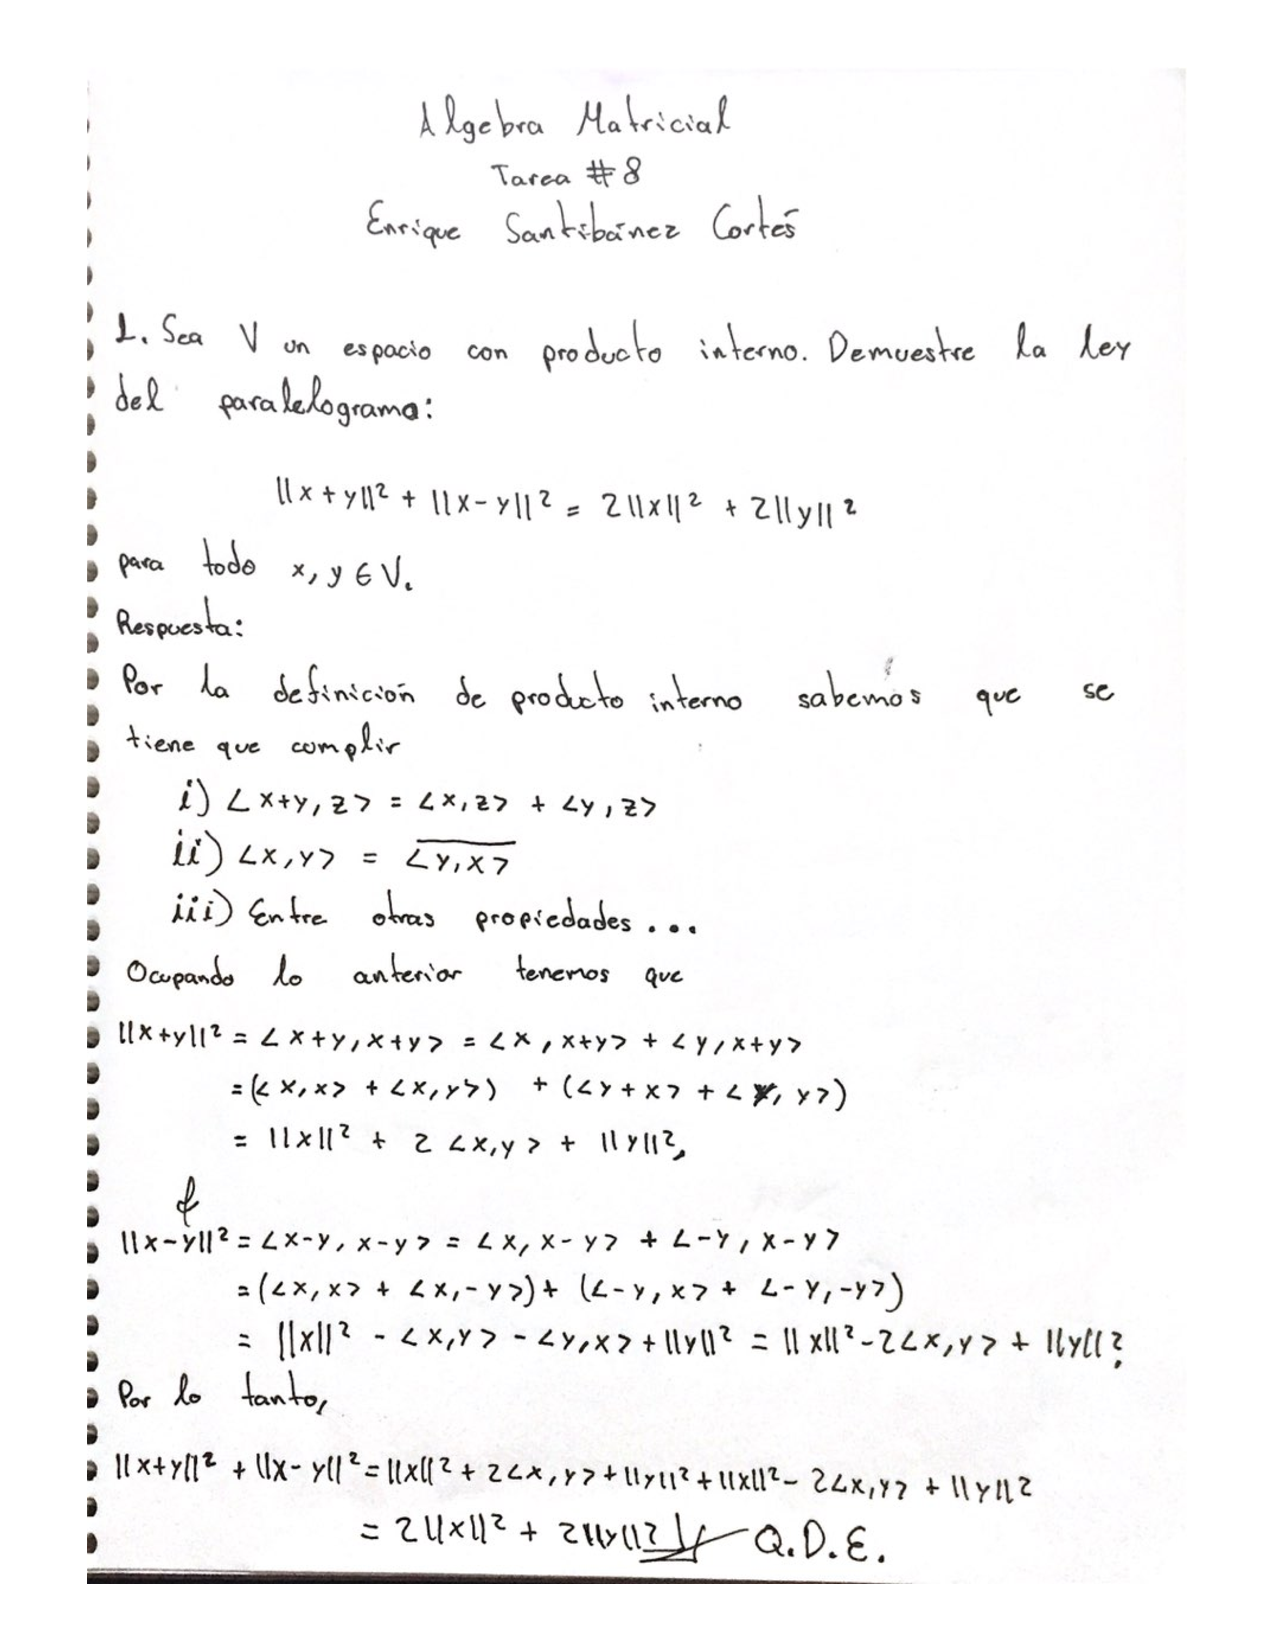
\includepdf[pages={1,2,3}]{ejercicios_mano.pdf}

\begin{table}[ht]
\centering
\begin{tabular}{c}
\textbf{Maestría en Computo Estadístico}\\
\textbf{Álgebra Matricial} \\
\textbf{Tarea 8}\\
\today \\
\emph{Enrique Santibáñez Cortés}\\
Repositorio de Git: \href{https://github.com/Enriquesec/Algebra_matricial/tree/master/tareas/Tarea_8}{Tarea 8, AM}.
\end{tabular}
\end{table}
Todos los cálculos deben ser a mano.

\begin{itemize}
\item[5.] Considere los vectores 
\begin{align*}
u_1=\begin{pmatrix} 1\\ 0 \\ 1 \end{pmatrix}, \ \ 
u_2=\begin{pmatrix} -1\\ 4 \\ 1 \end{pmatrix}, \ \ 
u_3=\begin{pmatrix} 2\\ 1 \\ -2 \end{pmatrix}.
\end{align*}
Demuestre que $\{u_1, u_2,u_3\}$ es una base ortogonal de $\mR^3$. Luego, exprese el vector 
\begin{align*}
v_1= \begin{pmatrix}
8\\
-4\\
-3
\end{pmatrix}
\end{align*}
como una combinación lineal de $u_1, u_2,u_3$. 

\res \begin{framed}
    \begin{thmd} \label{d_ortogonal}
	(Lemma 7.3, pag. 179 Linear Matriz,) Un conjunto de vectores $\{u_1 ,\cdots, u_p \}$ de $V$ se denomina conjunto ortogonal si cada par de vectores diferentes del conjunto es ortogonal, es decir, si $\langle u_i, u_j \rangle$ siempre
que $i \neq j$.
    \end{thmd}
\end{framed}

\begin{framed}
    \begin{thmt} \label{t_ortogonal}
	(Lemma 7.3, pag. 183 Linear Matriz,) Sea $S=\{u_1 ,\cdots, u_p \}$, es un conjunto ortogonal de vectores no nulos de $V$, entonces $S$ es linealmente independiente.
    \end{thmt}
\end{framed}

\begin{framed}
    \begin{thmt} \label{t_combinacion_lineal}
	(Visto en clase, pag. 148) Sea $V$ un espacio con producto interno y $W = \gen\{u_1 ,\cdots, u_p \}$, donde los $u_j$ forman un conjunto ortogonal de vectores en $V$ distintos de cero. Entonces $y\in W$ es de la forma
$$y=\alpha_1 u_1 + \cdots + \alpha_p u_p$$

donde
$$\alpha_j = \frac{\langle y, u_j \rangle}{\langle u_j, u_j \rangle}$$
    \end{thmt}
\end{framed}
Ocupemos la definición (\ref{d_ortogonal}) para probar que los vectores $u_i's$ son ortogonales, para ello calculemos el producto interno
\begin{align*}
\langle u_1, u_2 \rangle &= 1 (-1)+0(4)+1(1) = 0,\\
\langle u_1, u_3 \rangle &= 1(2) + 0(2)+1(-2)=0, \\
\langle u_2, u_3 \rangle &= -1(2)+4(1)+1(-2)=0.\\
\end{align*} 
Por lo tanto, como cada par de vectores $u_i's$ son ortogonales entonces podemos concluir que el conjunto $\{u_1, u_2,u_3\}$ es ortogonal. Ahora, por el teorema (\ref{t_ortogonal}) podemos concluir que el conjunto $\{u_1, u_2,u_3\}$ es linealmente independiente.  Como sabemos que $\dim(\mR^3)=3$ y también que $\#\{u_1, u_2,u_3\}=3$, entonces $\{u_1, u_2,u_3\}$ forma una base de $\mR^3$. Y por lo tanto, \textbf{podemos concluir que $\{u_1, u_2,u_3\}$ es una base ortogonal de $\mR^3$.}

Para expresar a $v_1$ como combinación lineal de $\{u_1, u_2,u_3\}$ ocupemos el teorema (\ref{t_combinacion_lineal}), primeros calculemos los productos puntos necesarios:
\begin{align*}
\langle u_1, u_1 \rangle &=& 1 (1)+0(0)+1(1) &=& 2,\ \ \ & \langle v_1, u_1 \rangle &=& 8(1)-4(0)-3(1) &=& 5\\
\langle u_2, u_2 \rangle &=& -1(-1) +4(4)+1(1)&=&18,\ \ \ & \langle v_1, u_2 \rangle &=& 8(-1) -4(4)-3(1)&=&-27,\\
\langle u_3, u_3 \rangle &=& 2(2)+1(1)-2(-2)&=&9,\ \ \ & \langle v_1, u_3 \rangle &=& 8(2)-4(1)-3(-2)&=&18.\\
\end{align*} 
Por lo tanto, el vector $v_1$ se puede expresar como combinación lineal de $\{u_1, u_2,u_3\}$ como
\begin{align*}
v_1&=\frac{5}{2} u_1+\frac{-27}{18}u_2+\frac{18}{9}u_3\\ \\
&=\bf \frac{5}{2}\begin{pmatrix} 1\\ 0 \\ 1 \end{pmatrix}+\frac{-3}{2}\begin{pmatrix} -1\\ 4 \\ 1 \end{pmatrix}
+2\begin{pmatrix} 2\\ 1 \\ -2 \end{pmatrix}.\ \ \ \finf
\end{align*}

\item[6.] Demuestre que el producto de matrices ortogonales es una matriz ortogonal.

\res \begin{framed}
    \begin{thmd} \label{d_matriz_ortogonal}
	(Visto en clase, pag. 155) Una matriz $U$ cuadrada es ortogonal si $UU^t=I.$
    \end{thmd}
\end{framed}
Demostremos por inducción que el producto de $n$ matrices ortogonales es otra matriz ortogonal.

\textbf{Paso 1:} Probarlo para $n=2$. Sea $A_1, A_2$ matrices ortogonales de tamaño $n\times n$, es decir, ocupando la definición \ref{d_matriz_ortogonal} tenemos que $A_iA_i^t=I, \ \ \i=1,2$. Sea $C$ la matriz resultante del producto de $A_1A_2$, entonces ocupando las propiedades básicas de la traza tenemos que 
\begin{align*}
CC^t=(A_1A_2)(A_1A_2)^T = (A_1A_2)(A_2^tA_1^t)= A_1(A_2 A_2^t)A_1^t=A_1IA_1^t=A_1A_1^t=I.
\end{align*}
Por lo tanto, podemos concluir que la matriz $C$ es ortogonal, es decir, el producto de $A_1$ y $A_2$ es ortogonal. 

\textbf{Paso 2:} Suponemos que se cumple para el producto de $n$ matrices ortogonales. Es decir, el producto de las matrices $A_1, A_2,...A_n$ ortogonales de tamaño $n\times n$, es otra matriz ortogonal.

\textbf{Paso 3:} Demostremos para $n+1$ matrices ortogonales. Sea $A_{n+1}$ otra matriz ortogonal de tamaño $n\times n$, ocupando el paso 2 tenemos que 
\begin{align*}
A_1A_2\cdots A_n A_{n+1}= (A_1A_2\cdots A_n)A_{n+1} = A'A_{n+1},
\end{align*}
donde $A'n$ es una matriz ortogonal. Y ocupando el paso $1$, como el producto de dos matrices ortogonales es otra ortogonal entonces podemos concluir que 
\begin{align*}
A_1A_2\cdots A_n A_{n+1}= (A_1A_2\cdots A_n)A_{n+1} = A'A_{n+1}= I.
\end{align*}
Es decir, queda demostrado que el producto de matrices ortogonales es otra matriz matriz ortogonal. \ \ \fin 


\item[7.] Dados los vectores
\begin{align*}
u_1=\begin{pmatrix} 3\\ -1 \\ 2 \end{pmatrix}, \ \ 
u_2=\begin{pmatrix} 1\\ -1 \\-2 \end{pmatrix}, \ \ 
y=\begin{pmatrix} -1\\ 2 \\ 6 \end{pmatrix}.
\end{align*}

i) Verifique que $u_1$ y $u_2$ son ortogonales, $ii)$ Encuentre la proyección ortogonal de $y$ sobre el espacio generado por $u_1$ y $u_2$.

\res \begin{framed}
    \begin{thmd} \label{d_proyeccion}
	(Definición 7.6, pag. 186 Linear Álgebra) Sea $v$ y $x$ dos vectores en $\mR^n$ tal que $v\neq 0$. Entonces, una proyección de $x$ sobre el vector $v$ viene dada por la función vectorial
	\begin{align*}
	proy_v(x)=\frac{\langle x, v \rangle}{\langle v,v \rangle} v.
	\end{align*}
	Por otro lado, la proyección ortogonal de $v$ sobre el
espacio $U$ generado por el conjunto de vectores ortogonales $\{u_1, . . . u_k\}$ no nulos se define como
$$proy_U (v) = proy_{u_1} (v) + proy_{u_2} (v) + \cdots + proy_{u_k} (v).$$
    \end{thmd}
\end{framed}

Tenemos que el producto interno de los vectores $u_1, u_2$ es
\begin{align*}
\langle u_1, u_2 \rangle= 3(1)-1(-1)+2(-2)=0.
\end{align*}
Por lo tanto, podemos concluir que \textbf{i) los vectores $u_1, u_2$ son ortogonales. } Ahora, ocupemos la definición (\ref{d_proyeccion}) para encontrar la proyección de $y$ en el espacio generado por $u_1, u_2$ para ello primero encontremos las proyeciones de $y$ en cada uno de los vectores $u_1, u_2$.
\begin{align*}
\langle u_1, u_1 \rangle &=& 3(3)-1(-1)+2(2) &=& 14,\ \ \ & \langle y, u_1 \rangle &=& -1(3)+2(-1)+6(2) &=& 7\\
\langle u_2, u_2 \rangle &=& 1(1)-1(-1)-2(-2)&=&6,\ \ \ & \langle y, u_2 \rangle &=& -1(1)+2(-1)+6(-2)&=&-15\Rightarrow
\end{align*} 
\begin{align*}
proy_{u_1}(y)=\frac{\langle y, u_1 \rangle}{\langle u_1,u_1 \rangle}=\frac{7}{14}\begin{pmatrix} 3\\ -1 \\ 2 \end{pmatrix}=\begin{pmatrix} 3/2\\ -1/2 \\ 1\end{pmatrix},\\
proy_{u_2}(y)=\frac{\langle y, u_2 \rangle}{\langle u_2,u_2 \rangle}=-\frac{15}{6}\begin{pmatrix} 1\\ -1 \\-2 \end{pmatrix}=\begin{pmatrix} -15/6\\ 15/6 \\ 5\end{pmatrix}.
\end{align*}
Por lo tanto, el proyección ortogonal de $y$ sobre el espacio generado por $u_1,u_2$ es
\begin{align*}
proy_U (y) = proy_{u_1}(y) + proy_{u_2}(y)=\begin{pmatrix} 3/2\\ -1/2 \\ 1\end{pmatrix}+ \begin{pmatrix} -15/6\\ 15/6 \\ 5\end{pmatrix} =\bf \begin{pmatrix}
-1\\ 2\\ 6
\end{pmatrix}. \ \ \ \finf
\end{align*}


\item[8.] Sea $W$ es espacio generado por 
\begin{align*}
u_1=\begin{pmatrix} 1\\ 1\\ 0 \\ 1 \end{pmatrix}, \ \ 
u_2=\begin{pmatrix} -1\\ 3 \\ 1 \\ -2\end{pmatrix}, \ \ 
u_3=\begin{pmatrix} -1\\ 0 \\ 1\\1 \end{pmatrix}.
\end{align*}
Si 
\begin{align*}
y=\begin{pmatrix}
4\\ 3\\ 3\\-1
\end{pmatrix}
\end{align*}
escriba $y$ como la suma de un vector en $W$ y un vector ortogonal a $W$.

\res \begin{framed}
    \begin{thmt} \label{t_suma}
	(Diapositiva pag. 149) Sea $V$ un espacio con producto interno y $W \subset V$ un subespacio. Entonces cualquier $y\in V$ se puede escribir de manera única como $$y=w+z$$ donde $w\in W$ y $z\in W^\perp$. Más aún, si $\{ u_1, \cdots, u_p\}$ es una base ortogonal de $W$, entonces
	\begin{align*}
	w=proy_{u_1}(y)+\cdots+proy_{u_p}(y) \ \ \ \& \ \ \ z=y-w.
	\end{align*}
    \end{thmt}
\end{framed}
Ocupemos la definición (\ref{d_ortogonal}) para probar que los vectores $u_i's$ son ortogonales, para ello calculemos el producto interno
\begin{align*}
\langle u_1, u_2 \rangle &= 1(-1) +1(3)+0(1)+1(-2) = 0,\\
\langle u_1, u_3 \rangle &= 1(-1) + 0(1)+1(0)+1(1)=0, \\
\langle u_2, u_3 \rangle &= -1(-1)+3(0)+1(1)-2(1)=0.
\end{align*} 
Por lo tanto, como cada par de vectores $u_i's$ son ortogonales entonces podemos concluir que el conjunto $\{u_1, u_2,u_3\}$ es ortogonal. Ahora, por el teorema (\ref{t_ortogonal}) podemos concluir que el conjunto $\{u_1, u_2,u_3\}$ es linealmente independiente. Entonces podemos concluir que $\{u_1, u_2, u_3\}$ es una base ortogonal para $W$. Ahora, encontremos las proyeciones de $y$ en cada uno de los vectores $u_1, u_2, u_3$.
\begin{align*}
\langle u_1, u_1 \rangle &=& 1(1)+1(1)+0(0)+1(1) &=&3,\ \ \ & \langle y, u_1 \rangle &=& 4(1)+3(1)+3(0)-1(1) &=&6\\
\langle u_2, u_2 \rangle &=& -1(-1)+3(3)+1(1)-2(-2)&=&15,\ \ \ & \langle y, u_2 \rangle &=& 4(-1)+3(3)+3(1)-1(-2)&=&10\\
\langle u_2, u_2 \rangle &=& -1(-1)+0(0)+1(1)+1(1)&=&3,\ \ \ & \langle y, u_2 \rangle &=& 4(-1)+3(0)+3(1)-1(1)&=&-2 \Rightarrow
\end{align*} 
\begin{align*}
proy_{u_1}(y)=\frac{\langle y, u_1 \rangle}{\langle u_1,u_1 \rangle}=\frac{6}{3}\begin{pmatrix} 1\\1\\0\\1 \end{pmatrix}=\begin{pmatrix} 2\\2\\0\\2 \end{pmatrix},\\
proy_{u_2}(y)=\frac{\langle y, u_2 \rangle}{\langle u_2,u_2 \rangle}=\frac{10}{15}\begin{pmatrix}-1\\3\\1\\-2 \end{pmatrix}=\begin{pmatrix} -2/3\\ 2\\2/3\\-4/3\end{pmatrix}\\
proy_{u_3}(y)=\frac{\langle y, u_2 \rangle}{\langle u_2,u_2 \rangle}=-\frac{2}{3}\begin{pmatrix}-1\\0\\1\\1 \end{pmatrix}=\begin{pmatrix} 2/3\\0\\-2/3\\-2/3 \end{pmatrix}.
\end{align*}
Por lo que, el proyección ortogonal de $y$ sobre el espacio generado por $u_1,u_2, u_3$ es
\begin{align*}
w = proy_{u_1}(y) + proy_{u_2}(y)+proy_{u_3}(y)=\begin{pmatrix} 2\\2\\0\\2 \end{pmatrix}+\begin{pmatrix} -2/3\\ 2\\2/3\\-4/3\end{pmatrix}+\begin{pmatrix} 2/3\\0\\-2/3\\-2/3 \end{pmatrix}=\begin{pmatrix}
2\\ 4 \\ 0 \\ 0
\end{pmatrix}.
\end{align*}
Entonces esto implica que 
\begin{align*}
z= y-w=\begin{pmatrix}
4\\ 3\\ 3\\-1
\end{pmatrix}-\begin{pmatrix}
2\\ 4 \\ 0 \\ 0
\end{pmatrix} = \begin{pmatrix} 2\\ -1\\ 3 \\ -1
\end{pmatrix}.
\end{align*}
Por lo tanto, $y$ se puede expresar como la suma de los vectores $w, y$ tal que $w\in W$ y $y\in W\perp$, es decir
$$\begin{pmatrix}
4\\ 3\\ 3\\-1
\end{pmatrix}=y = w+z=\begin{pmatrix}
2\\ 4 \\ 0 \\ 0
\end{pmatrix}+\begin{pmatrix} 2\\ -1\\ 3 \\ -1
\end{pmatrix}. \ \ \finf$$

\item[9.] Sea $W$ el espacio generado por 
\begin{align*}
u_1=\begin{pmatrix} 3\\1\\ -1 \\ 1 \end{pmatrix}, \ \ 
u_2=\begin{pmatrix} 1\\-1\\ 1 \\ -1 \end{pmatrix}.
\end{align*}
Si 
\begin{align*}
y =\begin{pmatrix}
3\\1\\5\\1
\end{pmatrix}
\end{align*}
encuentre el punto en $W$ más cercano a $y$.

\res \begin{framed}
    \begin{thmt} \label{t_cercano}
	(Diapositiva pag. 151) Sea $V$ un espacio con producto interno, $W \subset V$ un subespacio, $y \in V$ y $u = proy_W (y)$. Entonces $u$ es el vector en $W$ más cercano
a $y$.
    \end{thmt}
\end{framed}
Ocupando el teorema (\ref{t_cercano}) podemos encontrar el punto más cercano de $W$ a $y$. Primero verifiquemos que $u_1, u_2$ son ortogonales, calculemos el producto interno de los vectores $u_1, u_2$
\begin{align*}
\langle u_1, u_2 \rangle= 3(1)+1(-1)-1(1)+1(-1)=0.
\end{align*}
Por lo anterior, podemos concluir que $u_1, u_2$ son ortogonales. Ahora, ocupemos la definición (\ref{d_proyeccion}) para encontrar la proyección de $y$ en el espacio generado por $u_1, u_2$ para ello primero encontremos las proyeciones de $y$ en cada uno de los vectores $u_1, u_2$.
\begin{align*}
\langle u_1, u_1 \rangle &=& 3(3)+1(1)-1(-1)+1(1) &=&12,\ \ \ & \langle y, u_1 \rangle &=& 3(3)+1(1)+5(-1)+1(1) &=&6\\
\langle u_2, u_2 \rangle &=& 1(1)-1(-1)+1(1)-1(-1)&=&4,\ \ \ & \langle y, u_2 \rangle &=& 3(1)+1(-1)+5(1)+1(-1)&=&6 \Rightarrow
\end{align*} 
\begin{align*}
proy_{u_1}(y)=\frac{\langle y, u_1 \rangle}{\langle u_1,u_1 \rangle}=\frac{6}{12}\begin{pmatrix} 3\\ 1 \\ -1\\1 \end{pmatrix}=\begin{pmatrix} 3/2\\ 1/2 \\ -1/2\\1/2 \end{pmatrix},\\
proy_{u_2}(y)=\frac{\langle y, u_2 \rangle}{\langle u_2,u_2 \rangle}=\frac{3}{2}\begin{pmatrix} 1\\ -1 \\1\\-1 \end{pmatrix}=\begin{pmatrix} \frac{3}{2}\\ -\frac{3}{2} \\\frac{3}{2}\\-\frac{3}{2} \end{pmatrix}.
\end{align*}
Por lo que, el proyección ortogonal de $y$ sobre el espacio generado por $u_1,u_2$ es
\begin{align*}
proy_W (y) = proy_{u_1}(y) + proy_{u_2}(y)=\begin{pmatrix} 3/2\\ 1/2 \\ -1/2\\1/2 \end{pmatrix} + \begin{pmatrix} \frac{3}{2}\\ -\frac{3}{2} \\\frac{3}{2}\\-\frac{3}{2} \end{pmatrix} =\bf \begin{pmatrix}
3\\ -1 \\ 1\\ -1
\end{pmatrix}.
\end{align*}
Por lo tanto, \textbf{podemos concluir que el punto en $W$ más cercano a $y$ es $\bf \begin{pmatrix}
3\\ -1 \\ 1\\ -1
\end{pmatrix}$.}\ \ \ \fin

\item[10.] Encuentre una base ortogonal para el espacio columna de la matriz 
\begin{align*}
\begin{pmatrix}
3 & -5 &1\\
1 & 1 & 1\\
-1 & 5 &-2\\
3 & -7 & 8
\end{pmatrix}
\end{align*}

\res \begin{framed}
    \begin{thmd} \label{d_gram_schmidt}
	(Vista en clase) Gram-Schmidt. Sea una base $\{v_1,\cdots, v_p\}$ del subespacio $S$ de $V$. Definimos:
	\begin{align*}
	w_1 &= v_1,\\
	w_2 &= v_2-\frac{\langle v_2, w_1 \rangle}{\langle w_1,w_1 \rangle}w_1, \\
	\vdots\\
	w_p &= v_p-\frac{\langle v_p, w_1 \rangle}{\langle w_1,w_1 \rangle}w_1-\frac{\langle v_p, w_2 \rangle}{\langle w_2,w_2 \rangle}w_2-\cdots-\frac{\langle v_p, w_p \rangle}{\langle w_p,w_p \rangle}w_p.
	\end{align*}
	Entonces $\{w_1, \cdots, w_p\}$ es una base ortogonal de $S$. 
    \end{thmd}
\end{framed}
Primero encontremos una base para el espacio columna de $A$, ocupamos eliminación gaussiana para determinar si los vectores son linealmente independientes. 
\begin{align*}
&\begin{pmatrix}
3 & -5 &1\\
1 & 1 & 1\\
-1 & 5 &-2\\
3 & -7 & 8
\end{pmatrix}%
\grstep[R_3\Rightarrow R_3+R_1/3]{R_2 \Rightarrow R_2-R_1/3}
%
\begin{pmatrix}
3 & -5 & 1 \\
0 & \frac{8}{3} & \frac{2}{3} \\
0 & \frac{10}{3} & \frac{-5}{3} \\
3 & -7 & 8
\end{pmatrix}%
\grstep[R_2\Rightarrow 3R_2/8]{R_4 \Rightarrow R_4-R_1}
%
\begin{pmatrix}
3 & -5 & 1 \\
0 & 1 & 1/4 \\
0 & \frac{10}{3} & \frac{-5}{3} \\
0 & -2 & 7
\end{pmatrix}%
\grstep[R_3\Rightarrow 3R_3/10]{R_4 \Rightarrow R_4+2R_2}\\
&\begin{pmatrix}
3 & -5 & 1 \\
0 & 1 & 1/4 \\
0 & 1 & -1/2 \\
0 & 0 & 15/2
\end{pmatrix}%
\grstep[R_4\Rightarrow 2R_4/15]{R_3 \Rightarrow R_3-R_2}
%
\begin{pmatrix}
3 & -5 & 1 \\
0 & 1 & 1/4 \\
0 & 0 & -3/4 \\
0 & 0 & 1
\end{pmatrix}%
\grstep[R_4\Rightarrow R_4-R_3]{R_3 \Rightarrow -4R_3/3}
%
\begin{pmatrix}
3 & -5 & 1 \\
0 & 1 & 1/4 \\
0 & 0 & 1 \\
0 & 0 & 0
\end{pmatrix}
\end{align*}
Por lo anterior, podemos concluir que las columnas de $A$ son  vectores linealmente independientes por lo que una base para $A$ es
\begin{align*}
\mcC(A)=\gen\{a_1,a_2,a_3\}, \text{   donde } a_i \text{ son las columnas de A}.
\end{align*} 
Ahora, veamos si los vectores son vectores ortogonales. Para ello ocupemos la definición (\ref{d_ortogonal}) para probar que los vectores $u_i's$ verificar si son o no son ortogonales, para ello calculemos sus productos internos
\begin{align*}
\langle a_1, a_2 \rangle &= 3(-5) +1(1)-1(5)+3(-7)=-40\neq 0,\\
\langle a_1, a_3 \rangle &= 3(1) +1(1)-1(-2)+3(8)=30\neq 0, \\
\langle a_2, a_3 \rangle &= -5(1)+1(1)+5(-2)-7(8)=-70\neq 0.
\end{align*} 
Por lo tanto, podemos concluir que el conjunto $\{a_1, a_2,a_3\}$ es no es ortogonal y por ende no es una base ortogonal. Entonces ocupemos la metodología de Gram-Schmidt (\ref{d_gram_schmidt}) para transforma la base a una base ortogonal, 
\begin{align*}
w_1& = a_1,\\
w_2 &= a_2-\frac{\langle a_2, w_1 \rangle}{\langle w_1,w_1 \rangle}w_1,
\end{align*}
calculemos lo anterior 
\begin{align*}
\langle w_1, w_1 \rangle &=& 3(3)+1(1)-1(-1)+3(3)&=&20,\ \ \ & \langle a_2, w_1 \rangle &=& \langle a_2, a_1 \rangle &=&-40\Rightarrow
\end{align*}
\begin{align*}
w_2= \begin{pmatrix}
-5\\ 1\\5\\-7
\end{pmatrix}-\frac{-40}{20}\begin{pmatrix}
3\\ 1 \\-1\\3
\end{pmatrix}=\begin{pmatrix}
-5\\ 1\\5\\-7
\end{pmatrix}+\begin{pmatrix}
6\\ 2 \\-2\\6
\end{pmatrix}=\begin{pmatrix}
1\\ 3 \\3\\-1
\end{pmatrix}.
\end{align*}
Ahora,
\begin{align*}
w_3 &= a_3-\frac{\langle a_3, w_1 \rangle}{\langle w_1,w_1 \rangle}w_1-\frac{\langle a_3, w_2 \rangle}{\langle w_2,w_2 \rangle}w_2,
\end{align*}
calculemos lo anterior
\begin{align*}
\langle w_2, w_2 \rangle &=& 1(1)+3(3)+3(3)-1(-1)&=&20,\ \ \ & \langle a_3, w_2 \rangle &=& 1(1)+1(3)-2(3)+8(-1) &=&-10\\
\langle a_3, w_1 \rangle &=& \langle a_3, a_1 \rangle &=&30\Rightarrow
\end{align*}
\begin{align*}
w_3= \begin{pmatrix}
1\\1\\-2\\8
\end{pmatrix}-\frac{30}{20}\begin{pmatrix}
3\\ 1 \\-1\\3
\end{pmatrix}-\frac{-10}{20}\begin{pmatrix}
1\\3\\3\\-1
\end{pmatrix}=\begin{pmatrix}
1\\1\\-2\\8
\end{pmatrix}-\begin{pmatrix}
9/2\\ 3/2 \\-3/2\\9/2
\end{pmatrix}+\begin{pmatrix}
1/2\\ 3/2 \\3/2\\-1/2
\end{pmatrix}=\begin{pmatrix}
-3\\1\\1\\3
\end{pmatrix}.
\end{align*}
Por lo tanto, \textbf{una base ortogonal para el espacio columna de A es }
\begin{align*}
\left\{\begin{pmatrix}
3\\ 1\\-1\\3
\end{pmatrix} ,\begin{pmatrix}
1\\ 3 \\3\\-1
\end{pmatrix},\begin{pmatrix}
-3\\1\\1\\3
\end{pmatrix}\right\}. \ \ \finf
\end{align*}

\item[11.] Encuentre una descomposición $QR$ de 
\begin{align*}
A=\begin{pmatrix}
-1 & 6 & 6\\
 3 &-8 & 3\\
 1 &-2 & 6\\
 1 &-4 &-3 
\end{pmatrix}
\end{align*}

\res \begin{framed}
    \begin{thmd} \label{d_qr}
	(Definición 7.9, pag. 195) Si $A$ es una matriz $m \times n$ con columnas linealmente independientes, entonces $A$
puede ser factorizada de la forma $A = Q R$, donde $Q$ es una matriz $m \times n$ cuyas columnas forman una base ortonormal de $\mcC(A)$ y $R$ es una matriz $n\times n$ triangular
superior e invertible con componentes positivas en su diagonal principal.
    \end{thmd}
\end{framed}
Por la definición \ref{d_qr} sabemos que las columnas de $Q$ son forman una base ortonormal de $\mcC(A).$ Entonces empecemos por encontrar una base $\mcC(A)$,
\begin{align*}
&\begin{pmatrix}
-1 & 6 & 6\\
 3 &-8 & 3\\
 1 &-2 & 6\\
 1 &-4 &-3 
\end{pmatrix}%
\grstep[R_3\Rightarrow R_3+R_1]{R_2 \Rightarrow R_2+3R_1}
%
\begin{pmatrix}
-1 & 6 & 6 \\
0 & 10 & 21 \\
0 & 8 & 12 \\
1 & -4 & -3
\end{pmatrix}%
\grstep[R_3\Rightarrow R_3-4R_2/5]{R_4 \Rightarrow R_4+R_1}
%
\begin{pmatrix}
-1 & 6 & 6 \\
0 & 10 & 21 \\
0 & 0 & \frac{-24}{5} \\
0 & 2 & 3
\end{pmatrix}%
\grstep[]{R_4 \Rightarrow R_4-R_2/5}\\
&\begin{pmatrix}
-1 & 6 & 6 \\
0 & 10 & 21 \\
0 & 0 & \frac{-24}{5} \\
0 & 0 & \frac{-6}{5}
\end{pmatrix}%
\grstep[]{R_4 \Rightarrow R_4-R_3/4}
%
\begin{pmatrix}
-1 & 6 & 6 \\
0 & 10 & 21 \\
0 & 0 & \frac{-24}{5} \\
0 & 0 & 0
\end{pmatrix}.
\end{align*}
Por lo anterior, podemos concluir que las columnas de $A$ son  vectores linealmente independientes por lo que una base para $A$ es
\begin{align*}
\mcC(A)=\gen\{a_1,a_2,a_3\}, \text{   donde } a_i \text{ son las columnas de A}.
\end{align*} 
Ahora, veamos si los vectores son vectores ortogonales. Para ello ocupemos la definición (\ref{d_ortogonal}) para probar que los vectores $u_i's$ verificar si son o no son ortogonales, para ello calculemos sus productos internos
\begin{align*}
\langle a_1, a_2 \rangle &=-1(6)+3(-8)+1(-2)+1(-4)=-36\neq 0,\\
\langle a_1, a_3 \rangle &=-1(6)+3(3)+1(6)+1(-3)=6\neq 0, \\
\langle a_2, a_3 \rangle &= 6(6)-8(3)-2(6)-4(-3)=12\neq 0.
\end{align*} 
Por lo tanto, podemos concluir que el conjunto $\{a_1, a_2,a_3\}$ es no es ortogonal y por ende no es una base ortogonal. Entonces ocupemos la metodología de Gram-Schmidt (\ref{d_gram_schmidt}) para transforma la base a una base ortogonal, 
\begin{align*}
w_1& = a_1,\\
w_2 &= a_2-\frac{\langle a_2, w_1 \rangle}{\langle w_1,w_1 \rangle}w_1,
\end{align*}
calculemos lo anterior 
\begin{align*}
\langle w_1, w_1 \rangle &=& -1(-1)+3(3)+1(1)+1(1)&=&12,\ \ \ & \langle a_2, w_1 \rangle &=& \langle a_2, a_1 \rangle &=&-36\Rightarrow
\end{align*}
\begin{align*}
w_2= \begin{pmatrix}
6\\-8\\-2\\-4
\end{pmatrix}-\frac{-36}{12}\begin{pmatrix}
-1\\3\\1\\1
\end{pmatrix}=\begin{pmatrix}
6\\-8\\-2\\-4
\end{pmatrix}+\begin{pmatrix}
-3\\9\\3\\3
\end{pmatrix}=\begin{pmatrix}
3\\1\\1\\-1
\end{pmatrix}.
\end{align*}
Ahora,
\begin{align*}
w_3 &= a_3-\frac{\langle a_3, w_1 \rangle}{\langle w_1,w_1 \rangle}w_1-\frac{\langle a_3, w_2 \rangle}{\langle w_2,w_2 \rangle}w_2,
\end{align*}
calculemos lo anterior
\begin{align*}
\langle w_2, w_2 \rangle &=& 3(3)+1(1)+1(1)-1(-1)&=&12,\ \ \ & \langle a_3, w_2 \rangle &=& 6(3)+3(1)+6(1)-3(-1) &=&30\\
\langle a_3, w_1 \rangle &=& \langle a_3, a_1 \rangle &=&6\Rightarrow
\end{align*}
\begin{align*}
w_3= \begin{pmatrix}
6\\3\\6\\-3
\end{pmatrix}-\frac{6}{12}\begin{pmatrix}
-1\\3\\1\\1
\end{pmatrix}-\frac{30}{12}\begin{pmatrix}
3\\1\\1\\-1
\end{pmatrix}=\begin{pmatrix}
6\\3\\6\\-6
\end{pmatrix}-\begin{pmatrix}
1/2\\-3/2\\-1/2\\-1/2
\end{pmatrix}+\begin{pmatrix}
-15/2 \\ -5/2\\ -5\/2\\ -5/2
\end{pmatrix}=\begin{pmatrix}
-1\\-1\\3\\-1
\end{pmatrix}.
\end{align*}
Por lo tanto, una base ortogonal de $\mcC(A)$ sería
\begin{align*}
\left\{\begin{pmatrix}
-1\\3\\1\\1
\end{pmatrix} ,\begin{pmatrix}
3\\1\\1\\-1
\end{pmatrix},\begin{pmatrix}
-1\\-1\\3\\-1
\end{pmatrix}\right\}.
\end{align*}
Ahora normalizamos cada vector para obtener una base ortonormal,
\begin{align*}
&\frac{w_1}{\sqrt{\langle w_1, w_1 \rangle}} = \frac{1}{\sqrt{12}}\begin{pmatrix}
-1\\3\\1\\1
\end{pmatrix} = \begin{pmatrix}
-\frac{1}{2\sqrt{3}}\\\frac{3}{2\sqrt{3}}\\\frac{1}{2\sqrt{3}}\\\frac{1}{2\sqrt{3}}
\end{pmatrix}, \ \frac{w_2}{\sqrt{\langle w_2, w_2 \rangle}} = \frac{1}{\sqrt{12}}\begin{pmatrix}
3\\1\\1\\-1
\end{pmatrix} = \begin{pmatrix}
\frac{3}{2\sqrt{3}}\\\frac{1}{2\sqrt{3}}\\ \frac{1}{2\sqrt{3}}\\ -\frac{1}{2\sqrt{3}}
\end{pmatrix},\\
&\frac{w_3}{\sqrt{\langle w_3, w_3 \rangle}} = \frac{1}{\sqrt{12}}\begin{pmatrix}
-1\\-1\\3\\-1
\end{pmatrix} = \begin{pmatrix}
-\frac{1}{2\sqrt{3}}\\ -\frac{1}{2\sqrt{3}}\\ \frac{3}{2\sqrt{3}} \\ -\frac{1}{2\sqrt{3}}
\end{pmatrix}.
\end{align*}
Por lo anterior, podemos concluir que 
\begin{align*}
Q= \begin{pmatrix}
-\frac{1}{2\sqrt{3}}& \frac{3}{2\sqrt{3}} &-\frac{1}{2\sqrt{3}}\\
\frac{3}{2\sqrt{3}} & \frac{1}{2\sqrt{3}} &-\frac{1}{2\sqrt{3}}\\
\frac{1}{2\sqrt{3}} & \frac{1}{2\sqrt{3}} & \frac{3}{2\sqrt{3}}\\
\frac{1}{2\sqrt{3}} & -\frac{1}{2\sqrt{3}}&-\frac{1}{2\sqrt{3}}
\end{pmatrix} = \frac{1}{2\sqrt{3}}\begin{pmatrix}
-1 & 3 &-1\\
3 & 1 & -1\\
1& 1 & 3\\
1 & -1 & -1
\end{pmatrix}.
\end{align*}
Puesto que las columnas de $Q$ son ortonormales, tenemos que $Q^tQ = I$. Ahora necesitamos encontrar la matriz triangular superior $R$ que verifica $A = Q R$. Si multiplicamos ambos miembros de esta expresión por $Q^t$ resulta
\begin{align*}
Q^t A = Q^t QR=IR=R.
\end{align*}
Así,
\begin{align*}
R&= Q^t A = \frac{1}{2\sqrt{3}}\begin{pmatrix}
-1 & 3 &-1\\
3 & 1 & -1\\
1& 1 & 3\\
1 & -1 & -1
\end{pmatrix}^t \begin{pmatrix}
-1 & 6 & 6\\
 3 &-8 & 3\\
 1 &-2 & 6\\
 1 &-4 &-3 
\end{pmatrix} = \frac{1}{2\sqrt{3}}\begin{pmatrix}
-1 & 3 & 1 & 1\\
 3 & 1 & 1 & -1\\
-1 &-1 & 3 & -1
\end{pmatrix}^t \begin{pmatrix}
-1 & 6 & 6\\
 3 &-8 & 3\\
 1 &-2 & 6\\
 1 &-4 &-3 
\end{pmatrix}\\
&= \frac{1}{2\sqrt{3}}\left(\begin{matrix}
1+9+1+1 & -6-24-2-4 & -6+9+6-3 \\
-3+3+1-1 & 18-8-2+4 & 18+3+6+3\\
1-3+3+1 & -6+8-6+4 & -6-3+18+-3
\end{matrix}\right) = \frac{1}{2\sqrt{3}}\left(\begin{matrix}
12 & -36 & 6 \\
0 & 12 & 30 \\
0 & 0 & 12
\end{matrix}\right)\\
&= \begin{pmatrix}
6/\sqrt{3} & -18/\sqrt{3} & 3/\sqrt{3} \\
0 & 6/\sqrt{3} & 15/\sqrt{3} \\
0 & 0 & 6/\sqrt{3}
\end{pmatrix} = \begin{pmatrix}
2\sqrt{3} & -6\sqrt{3} & \sqrt{3} \\
0 & 2\sqrt{3} & 5\sqrt{3} \\
0 & 0 & 2\sqrt{3}
\end{pmatrix}.
\end{align*}
Por lo tanto, \textbf{la descomposición $QR$ de $A$ es}
\begin{align*}
A=\begin{pmatrix}
-1 & 6 & 6\\
 3 &-8 & 3\\
 1 &-2 & 6\\
 1 &-4 &-3 
\end{pmatrix}=\begin{pmatrix}
-\frac{1}{2\sqrt{3}}& \frac{3}{2\sqrt{3}} &-\frac{1}{2\sqrt{3}}\\
\frac{3}{2\sqrt{3}} & \frac{1}{2\sqrt{3}} &-\frac{1}{2\sqrt{3}}\\
\frac{1}{2\sqrt{3}} & \frac{1}{2\sqrt{3}} & \frac{3}{2\sqrt{3}}\\
\frac{1}{2\sqrt{3}} & -\frac{1}{2\sqrt{3}}&-\frac{1}{2\sqrt{3}}
\end{pmatrix}  \begin{pmatrix}
2\sqrt{3} & -6\sqrt{3} & \sqrt{3} \\
0 & 2\sqrt{3} & 5\sqrt{3} \\
0 & 0 & 2\sqrt{3}
\end{pmatrix}=QR.\ \ \finf
\end{align*}
\item[12.] Encuentre las soluciones de mínimos cuadrados de $Ax=b$ con 
\begin{align*}
A=\begin{pmatrix}
 1 & -2\\
-1 &  2\\
 0 &  3\\
 2 &  5
\end{pmatrix}, \ \ b=\begin{pmatrix}
3\\ 1\\ -4\\2 
\end{pmatrix}.
\end{align*}

\res \begin{framed}
    \begin{thmt} \label{t_minimos}
	(Diapositiva pag. 157) Son equivalentes
	\begin{enumerate}
	\item La solución de mínimos cuadrados de $Ax = b$ es única.
	\item Las columnas de $A$ son linealmente independientes.
	\item $A^tA$ es invertible.
	\end{enumerate}
	En cualquier caso de los anteriores $$\hat{x}= (A^tA)^{-1} A^tb$$.
    \end{thmt}
\end{framed}
Ocupemos el teorema (\ref{t_minimos}), primero calculemos el siguiente producto
\begin{align*}
A^tA&=\begin{pmatrix}
1 & -1 & 0 & 2 \\
-2 & 2 & 3 & 5
\end{pmatrix} \begin{pmatrix}
 1 & -2\\
-1 &  2\\
 0 &  3\\
 2 &  5
\end{pmatrix} \\
&=\left(\begin{matrix}
1(1)+\left(-1\right)\left(-1\right)+0(0)+2(2) & 1\left(-2\right)+\left(-1\right)(2)+0(3)+2(5) \\
-2(1)+2\left(-1\right)+3(0)+5(2) & -2\left(-2\right)+2(2)+3(3)+5(5)
\end{matrix}\right)\\
&= \begin{pmatrix}
6 & 6 \\
6 & 42
\end{pmatrix}.
\end{align*}
Ahora, como $\det(A^t A) = \det \left(\begin{pmatrix}
6 & 6 \\
6 & 42
\end{pmatrix} \right) = 6(42)-6(6)=6(36)\neq 0$ podemos concluir que la matriz $A^t A$ es invertible. Entonces como $A^t A$ es invertible podemos concluir que la solución de mínimos cuadrados de $Ax=b$ es única y se encuentra como $(A^tA)^{-1}A^t b$. Ahora calculemos la inversa de $A^t A$ (se ocupa el teorema \ref{t_inversa}),
\begin{align*}
(A^tA)^{-1} = \begin{pmatrix}
6 & 6 \\
6 & 42
\end{pmatrix}^{-1} = \frac{1}{6(42)-6(6)}\begin{pmatrix}
42 & -6\\
-6 & 6
\end{pmatrix}=\left(\begin{matrix}
\frac{7}{36} & \frac{-1}{36} \\
\frac{-1}{36} & \frac{1}{36}
\end{matrix}\right).
\end{align*}
Entonces la solución de mínimos cuadrados de $Ax=b$ es
\begin{align*}
\hat{x}& = (A^tA)^{-1} A^tb = \left(\begin{matrix}
\frac{7}{36} & \frac{-1}{36} \\
\frac{-1}{36} & \frac{1}{36}
\end{matrix}\right) \begin{pmatrix}
1 & -1 & 0 & 2 \\
-2 & 2 & 3 & 5
\end{pmatrix}\begin{pmatrix}
3\\ 1\\ -4\\2 
\end{pmatrix}\\
&= \left(\begin{matrix}
\frac{7}{36} & \frac{-1}{36} \\
\frac{-1}{36} & \frac{1}{36}
\end{matrix}\right) \left(\begin{matrix}
1(3)+\left(-1\right)(1)+0\left(-4\right)+2(2) \\
-2(3)+2(1)+3\left(-4\right)+5(2)
\end{matrix}\right) \\
&= \left(\begin{matrix}
\frac{7}{36} & \frac{-1}{36} \\
\frac{-1}{36} & \frac{1}{36}
\end{matrix}\right) \begin{pmatrix}
6\\-6
\end{pmatrix}\\
&=\left(\begin{matrix}
\frac{7}{36}(6)+\frac{-1}{36}\left(-6\right) \\
\frac{-1}{36}(6)+\frac{1}{36}\left(-6\right)
\end{matrix}\right) \\
&=\left(\begin{matrix}
\frac{4}{3} \\
\frac{-1}{3}
\end{matrix}\right).
\end{align*}
Es decir, \textbf{el sistema $Ax=b$ tiene solución única y es $x=\left(\begin{matrix}
4/3 \\
-1/3
\end{matrix}\right)$} \ \ \ \fin


\textsc{Anexo:} 
\begin{framed}
    \begin{thmt} \label{t_inversa}
	(Recordatorio) Encontrar la inversa de una matriz A de $2\times 2$ mediante la fórmula
\begin{align*}
A^{-1}=\begin{pmatrix}
a & b\\
c & d
\end{pmatrix}^{-1}=\frac{1}{|A|}\begin{pmatrix}
C_{11} & C_{21}\\
C_{12} & C_{22}
\end{pmatrix}=\frac{1}{ad-bc}\begin{pmatrix}
d & -b\\
-c & a
\end{pmatrix}.
\end{align*}
    \end{thmt}
\end{framed}

Nota: Los primero 5 ejercicios ya no me dio tiempo pasarlos a latek, espero no sea complicado entenderle a mi letra. 

\end{itemize}
\end{document}